%%%%%%%%%%%%%%%%%%%%%%%%%%%%%%%%%%%%%%%%%%%%%%%%%%%%%%%%%%%%%%%%%%%%%%%%%%%%%%%%
%% Sample document ``thesis.tex''
%%

% Available documentclass options:
% - <all `report` document class options, e.g.: `a5paper`>
\documentclass[]{simple-thesis}


%%%%%%%%%%%%%%%%%%%%%%%%%%%%%%%%%%%%%%%%%%%%%%%%%%%%%%%%%%%%%%%%%%%%%%%%%%%%%%%%
%% Some mods
%%
\usepackage{graphicx}
\usepackage{courier}
\usepackage{listings}
\usepackage[margin=1cm]{caption}
\usepackage[toc]{appendix}
\usepackage{array}
\usepackage{float}
\newcolumntype{C}{>{\centering\arraybackslash}p{1.5cm}}
\renewcommand{\labelitemii}{$\circ$}  % Set the nested itemize style to empty circle.
\lstset{
  basicstyle=\footnotesize\ttfamily,
  numbers=left
}
\newcommand\fnurl[2]{%
  \href{#2}{#1}\footnote{\url{#2}}%
}


%%%%%%%%%%%%%%%%%%%%%%%%%%%%%%%%%%%%%%%%%%%%%%%%%%%%%%%%%%%%%%%%%%%%%%%%%%%%%%%%
%% Thesis meta-information
%%

%% The title of the thesis:
\title{UnsocialVR: Faking active listening in social virtual environments}

%% The full name of the author (e.g.: James Smith):
\author{Tom Gurion}

%% Affiliation:
\affiliation{Media and Arts Technology\\Queen Mary University of London}
\affiliationlogo{CollegeShields/QMUL}

%% You can redefine the submission notice [optional]:
\submissionnotice{Advanced placement project final report\\Supervisor: Patrick Healey\\Host: Inition}

%% PDF meta-info:
\hypersetup{pdfsubject={TODO subject},pdfkeywords={TODO keywords}}


%%%%%%%%%%%%%%%%%%%%%%%%%%%%%%%%%%%%%%%%%%%%%%%%%%%%%%%%%%%%%%%%%%%%%%%%%%%%%%%%
%% Abstract:
%%
\abstract{%
  TODO abstract...
}


%%%%%%%%%%%%%%%%%%%%%%%%%%%%%%%%%%%%%%%%%%%%%%%%%%%%%%%%%%%%%%%%%%%%%%%%%%%%%%%%
%% Acknowledgements:
%%
\acknowledgements{%
  TODO acknowledgments...

  Patrick Healey.
  Inition.
  Pedro.
  Stuart.
}


%%%%%%%%%%%%%%%%%%%%%%%%%%%%%%%%%%%%%%%%%%%%%%%%%%%%%%%%%%%%%%%%%%%%%%%%%%%%%%%%
%% Contents:
%%
\begin{document}

\frontmatter{}  %% Title page, abstract, TOC, etc.


%%%%%%%%%%%%%%%%%%%%%%%%%%%%%%%%%%%%%%%%%%%%%%%%%%%%%%%%%%%%%%%%%%%%%%%%%%%%%%%%
%% Thesis body:
%%
\chapter{Introduction}

In Infinite Jest, David Foster Wallace argues that "Good old traditional audio-only phone conversations allowed you to presume that the person on the other end was paying complete attention to you while also permitting you not to have to pay anything even close to complete attention to her." \citep{Wallace1996}.
He continues and claims that we are addicted to this illusion, and that's why video conferencing always feel so awkward - we need to pretend to listen all the time.
And if we think about it, even in face to face conversation we must always adhere to these social rules, and signal our complete attention when someone is talking to us.

In this project I experiment with virtual reality (VR) technologies to see if this illusion of faking active listening is transferable to other mediums, and if so, how.
In Unsocial VR participants share the same virtual environment, using VR headsets and controllers.
They can converse freely and move around, and if they want to start faking listening to the conversation and just wander around, or even talk with other participants while faking, they absolutely can!
The interface is very minimal, just hit a button on the controller to start faking active listening behaviours towards your current conversation, and release it when you want to stop faking.
Players even get an on screen notification when someone is speaking directly to them, so they can return to the conversation elegantly.

TODO More generally...
Social VR as an environment to investigate behaviours.

Chapter \ref{literature_review} review the relevant literature on the topics relevant for the current study.
Chapter \ref{system_design_and_implementation} present the system developed for the study, including detailed motivation for each decision.
Chapter \ref{evaluation} show the evaluation of the system.
Chapter \ref{general_discussion} discuss the finding.
Chapter \ref{conclusions} conclude this report with TODO and suggestions for future work.


\chapter{Literature review}\label{literature_review}

This project is based on multidisciplinary research.
It merges ideas from telepresence and mediated communication, that explore the representation of non verbal cues in new communication technologies;
depends on multiparty social interaction analysis, which uses spatial cues to understand who is talking with whom in dynamic social environments;
make use of new ways to generate active listening cues, such as head nods, in automated agents;
and influenced by research in asymmetric social communication in virtual environments.

\section{Telepresence and mediated communication}

Surveys \citep{Isaacs1994, Erickson2000}.

Social VR.

The GAZE systems \citep{Vertegaal1999, Vertegaal2003}.

Transformed social interaction \citep{Bailenson2004, Bailenson2008}.

\section{Multiparty social interaction}

%% TODO is it worth adding a more general intro using \citep{Hall1966} and \citep{Goffman1966}?

Groups of people that interact in free standing conversations tend to form spatial clusters.
Understanding these clusters, also known as F-formations, have several applications ranging from surveillance, through social robotics, and, as demonstrated in this study, to social VR.
According to \citeauthor{Kendon1990} ``an F-formation arises whenever two or more people sustain a spatial and orientational relationship in which the space between them is one to which they have equal, direct, and exclusive access'' (\citeyear[p. 209]{Kendon1990}).
F-formations can take many shapes.
Common examples are circular, side-by-side, or L-shaped conversations.
An F-formations system, however, doesn't solely describe the spatial organization of participants in a social interaction.
It also implies a set of expected social behaviours.
An L-shaped interaction, for example, suggests TODO, whereas a circular interaction may TODO.
The most prominent spatial feature of an F-formation is probably its o-space: the area in the center of the cluster that captures the attention of the members in the F-formation.

Before moving to discuss ways to automate F-formation detection there are two definitions that are important to grasp.
The \textit{transactional segment} is the area in front of the body that can be reached easily and into which we look and speak.
The \textit{o-space} is the area that is surrounded by the members of the F-formation, and to which they have exclusive access.
The o-space is often describe by means of the transactional segment of the F-formation members, and can be seen as the area in which the transactional segments overlap.

Based on these characteristics, automatic detection of F-formations usually rely on the participants position and orientation.
Whereas the position in space is usually well defined, there are different approaches to understand orientation.
\citeauthor{Kendon1990} suggests that the orientation should be determined by the lower body (\citeyear{Kendon1990}).
When standing, for example, the orientation should be calculated based on the position of the feet.
He adds that this is not uncommon to rotate the head and look outside of the transactional segment.
These head rotations are usually temporary anyway, so F-formation analysis can ignore them.
In the case of actually moving the center of attention and transactional segment the head move will be followed by changing the lower body orientation as well.
This idea is inline with \citeauthor{Schegloff1998}'s understanding of body pose in conversation (\citeyear{Schegloff1998}).
In his paper, the \textit{home position} --- the sustained center of attention --- is defined by the lower body orientation.
An upper body rotation is inherently unstable situation that should be resolved by either changing the lower body orientation or by returning to the home position.
Recent empirical study provided evidence that F-formation are indeed best understood using lower body orientation by TODO (TODO find ref).
Regardless of these theoretical arguments and evidence, many studies use the head direction to analyze F-formations \citep{Cristani2011, Setti2013, Vascon2014}.
One possible reason is that most of these studies are done in the field of computer vision and it is harder to extract lower body information from video due to occlusion \citep{Yasuda2014, Vascon2014}.

Different methods were recently proposed for automating F-formation analysis.
\citeauthor{Lin2010} applied a hidden Markov model to model relationships between people in video surveillance context (\citeyear{Lin2010}).
In addition to group detection, their algorithm can detect hierarchical interactions and group activity.
\citeauthor{Hung2011} suggested an algorithm for F-formation detection based on dominant sets (\citeyear{Hung2011}).
They collected and annotated social interaction video footage, and compared the algorithm results to F-formation analysis that was done manually.
This dataset is still used in later studies to assess the performance of F-formation detection algorithms.
Another approach was presented by \citeauthor{Cristani2011} using a voting strategy based on the Hough transform (\citeyear{Cristani2011}).
A comparison of the previous two studies is provided by \cite{Setti2013}.
Recently, state of the art algorithms combine probabilistic approaches to model the transactional segment and present an even better predictive power compared to previous studies \citep{Vascon2014, Setti2015}.
\citeauthor{Vascon2014} used socio-psychological inspired model to represent biological constrains of social attention (\citeyear{Vascon2014}).
A game-theoretic framework embedded these constrained to find the most probable F-formations for the data.
Interestingly, they also integrated temporal information to reduce noise in the data and therefore get more robust predictions.
Lastly, \citeauthor{Setti2015} developed a similar model using graph cuts algorithm (\citeyear{Setti2015}).

It is important to note that most of the studies in F-formation detection are bounded to single-frame contexts.
F-formation systems, however, have temporal characteristics over time.
For example, members of an F-formation may come and go while the system, as an organization unit, might be preserved.
Moreover, the F-formation itself might move as it adapts to the change of members \citep{Kendon1990}.
In such cases, being able to track the F-formation over time might provide insights for the underlying social interaction.
In the context of the current research, and without sufficient literature and existing algorithms, a relatively simple algorithm is proposed for extending single-frame F-formations detection for continuous tracking.

\section{Active listening}

In order to make a conversation natural and engaging, conversing parties use a wide array of social cues.
These signals can indicate the parties interest in keeping the conversation going, show mutual understanding, or the attempt to take the speaker turn.
Whereas conversations are usually considered to be a lingual phenomena, many of these social signals are non-verbal (e.g.\ head nods and facial expressions), or extra-linguistic (e.g.\ utterances like ``uh-huh'').
In the context of active listening behaviours they are known as backchannels \citep{Yngve1970}.
They are important for establishing rapport \citep{Gratch2007} and have significant effect on the speaker behaviour \citep{Bavelas2000}.
Not surprisingly, one of the main application of backchannels research is the implementation of automated agents that can provide socially appropriate responses in free conversation \citep{Morency2008, Bevacqua2008}.
There are reasons to believe that backchannels can be predicted without attending the content of the conversation \citep{Yngve1970}.
Therefore, researchers consistently attempt to use surface features like speaker-listener eye contact, speaker voice level, and prosody to model backchannels.

\citeauthor{Ward2000} suggested a backchannel prediction model that is based on the speaker prosody (\citeyear{Ward2000}).
Their model used a small set of features and simple hand-crafted rules.
Specifically, speaker ``talking state'' (speaking or silent) and the pitch of the speaker voice were taken into account.
\citeauthor{Gratch2006} propose to incorporate the speaker head moves and body pose into a similar model (\citeyear{Gratch2006}).
Another approach is to use surface text features to model backchannels \citep{Lee2006}.
In this study, the model is based on a bag-of-words technique, with different spoken words triggering different listener responses.
They based their rules on manual analysis of video recorded conversations with embodied conversational agents.
All of these studies used a set of carefully chosen hand-crafted rules to build their backchannel prediction models.

Recent studies suggest that data-driven approaches for modeling backchannels improve the model performance.
\citeauthor{Nishimura2007} predict listener responses using the pitch and power of the speaker voice (\citeyear{Nishimura2007}).
Their model, however, isn't constrained to predict backchannels only.
A response generator uses audio features to choose between types of responses, like backchannels, collaborative completion (e.g. suggesting a keyword for the speaker), and more.
Their decision-tree model was trained using audio-recorded and annotated conversations of the RWC multimodal database \citep{Hayamizu1996}.
\citeauthor{Morency2008} followed a similar path but with a more exhaustive set of audio-based features, and speaker-listener gaze annotations (\citeyear{Morency2008}).
In addition, they encoded each feature with a set of encoding templates that modified the appearance of the feature over time.
Then, they applied probabilistic methods to choose the feature with the most predictive power to incorporate into the model.
\citeauthor{Huang2011} uses a simplified model that is based only on non-verbal information (\citeyear{Huang2011}).
Their model uses the speaker talking state, speaker-listener eye contact, and, interestingly, the speaker smile, to predict listener backchannels.
A year later, \citeauthor{Kok2012} suggested some improvements to the same model to make it more robust to different speaker behaviours (\citeyear{Kok2012}).
Note that there is almost no direct comparison between the different models, mainly due to the use of different datasets and different evaluation methods \citep{Morency2008}.

%% TODO decide if it's worth mentioning. Use \cite{Gratch2007} as a baseline.
%% Another interesting approach to elicit rapport with automated conversational agents is to use mimicry.
%% \citeauthor{Bailenson2005} found that an automated agent is perceived as more persuasive if it's mimicking the speaker movement with four seconds lag (\citeyear{Bailenson2005}).

Before ending this section, it is important to discuss the theoretical distinction between the different participants roles in a social interaction.
Some of the roles are more obvious, like the role of the speaker in a conversation.
The differences between other roles, however, might be harder to tell.
According to \citeauthor{Clark1982}, apart from the speaker, participants in a conversation can take a role of addressees, side-participants, and over-hearers (\citeyear{Clark1982}).
Put simply, addressees are the listeners that the speaker illocutionary act is directed to.
Side-participants are the listeners that the speaker wish to inform about his/her illocutionary act towards the addressees.
Although they usually not expected to take the floor, they are an important part of the conversation.
The speaker must take the side-participants understanding in mind, and expected confirmation for their understanding, probably through non verbal cues (TODO find ref).
Over-hearers are listeners that the speaker have no interest in them hearing the conversation.
They are less relevant for the current study and thus won't be further discussed.
The roles are usually assigned to the participants, implicitly, by the speaker.

Most of the current research in backchannels and active listening behaviour is concentrated on two party conversations.
Therefore, side-participants active listening behaviours are much less investigated, understood, and modeled.
TODO present \citep{Matsusaka2003, Fujie2009}.

\section{Asymmetric communication}

\citep{Chou2016, Yee2007, Dominguez2014}.


\chapter{System design and implementation}\label{system_design_and_implementation}

Whereas many studies explore active listening behaviours using embodied conversational agents (ECAs) \citep{Nishimura2007, Bevacqua2008, Gratch2007, Huang2011, Lee2006, Poppe2013}, the current research aim to investigate how humans can start to pretend to listen to someone, how they stop faking and return to the conversation, and what are the social implication for such behaviours.
Recently, social research see high opportunities in exploring social behaviours using virtual environments \citep{Bailenson2008}.
Following the same trend, and inspired by the possibilities to fake attention in ways that are impossible in face-to-face conversation, the current research is based on a social virtual environment system.

The main target of the system is to support exploration of faked active listening behaviours in a social context.
As such, it implements a shared virtual environment, and uses a minimal user interface to let participants start and stop faking active listening behaviour towards the conversational group they belong to.
In the background, a set of components analyze the social interaction and manipulate how each participant experience the environment.

Figure \ref{fig:system:diagram} shows a schematic diagram of the system, and the paths and protocols of communication between the components.
The components in blue represent client side code, those in green are the client facing servers, and the red ones are background servers that process behavioural data to instruct the client facing servers how to operate.
A thorough description of each component in the system is presented bellow.

The code-base for the entire project is open sourced and \fnurl{available online}{https://github.com/Nagasaki45/UnsocialVR}.

\begin{figure}
  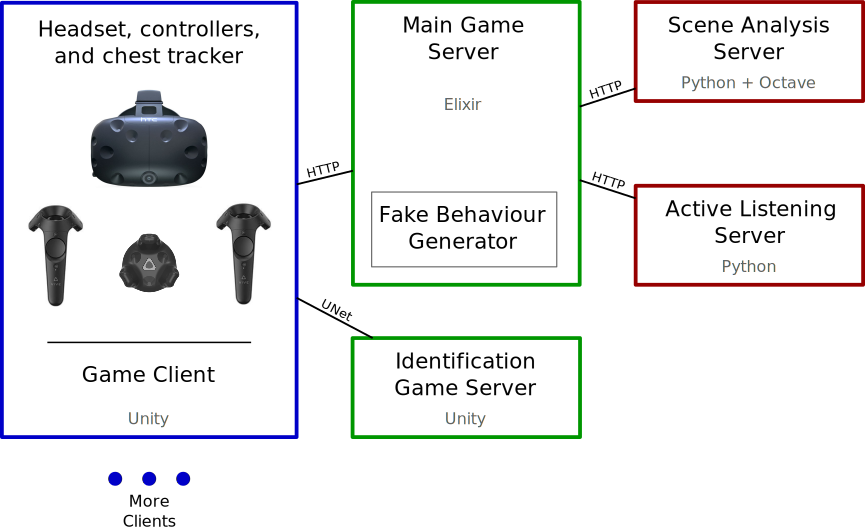
\includegraphics[width=\textwidth]{../graphics/system_diagram.pdf}
  \caption{A schematic diagram of the system architecture. In blue are client side components, that communicate with the client facing servers in green. The components in red are background servers that are used by the client facing servers to process behavioural data. The lines between the components represents paths of communication with the a label indicating the protocol.}
  \label{fig:system:diagram}
\end{figure}

\section{Hardware}

The hardware used in this project is the \fnurl{HTC Vive}{https://www.vive.com/uk/}, which bundle together a headset and two hand controllers.
In addition, \fnurl{Vive trackers}{https://www.vive.com/uk/vive-tracker/} are used to track the chest position of each participant.
This setup provided suitable features for the project compared to products like the \fnurl{Oculus Rift}{https://www.oculus.com/rift/}, or simpler VR solutions like \fnurl{Google Daydream}{https://vr.google.com/daydream/} or \fnurl{Samsung Gear VR}{http://www.samsung.com/global/galaxy/gear-vr/}.
Specifically, my system make use of the following features of the headset, that I couldn't find in other products:

\begin{itemize}
  \item The headset and its controllers and trackers are tracked in 3 dimensional (3D) space of up to 6 x 6 meters, enough for freely wondering around in a virtual environment. Recently, the Oculus Rift started to provide similar capabilities but they are better supported by the HTC Vive.
  \item The ability to combine extra trackers, that are used in this project to track the chest of the participant, are not available in other products.
\end{itemize}

\section{Game Client}

\begin{figure}
  \centering
  
\includegraphics[width=.5\textwidth]{../graphics/environment_demo.png}
  \caption{Example view of the virtual environment, showing the cocktail party context and the avatar design.}
  \label{fig:system:environment_demo}
\end{figure}

The Game Client is the application each participant use to connect to the 3D virtual environment.
Figure \ref{fig:system:environment_demo} shows how the virtual environment and the avatars look like.
I choose to contextualize the environment as a cocktail party on the beach.
This decision is mainly influenced by the intent to create a shared space where people can interact and dynamically form conversational groups.
Note that cocktail parties are common examples for such environments in the scientific literature \citep{Setti2015}.

Two main principles guided the design of the player avatar.
First, attempts to design a realistic avatar often elicit feelings of eeriness and revulsion.
This effect, also known as the \textit{uncanny valley}, suggests that when robots become more human like, our empathy to them increase.
It is true until a point of high similarity to humans where there is a ``valley'' in the empathy curve \citep{Mori1970}.
So, to stay away from the uncanny valley, I choose to design the avatar in a cartoon, unrealistic style.
This is inline with similar decision by commercial social VR products \citep{Ghosh2017, AltspaceVR2016, Pot2016}.
Second, with F-formation theory in mind, the avatar is made out of 4 body parts: head, 2 hands, and chest.
The visibility of the head and hands in the virtual environment immerses the players in the experience and makes the player more aware of their body.
The chest, however, is there mainly to signal the body orientation and therefore attention and sense of belonging to a conversation.
Originally, the cartoon style of the avatar made the orientation unclear.
To solve this, a belt with a buckle helps indicating the body direction.

Most of the 3D models were designed by me using \fnurl{blender}{https://www.blender.org/}.
I choose blender mainly because it is an open source project, whereas most of the alternatives are non-free commercial software.
Choosing a free and open source solution will allow me to reuse the acquired skills in future projects.

The players interface is minimal.
There is one button on the controller that when pressed, the player starts to fake active listening towards the other players in the same F-formation.
When the button is released the faked behaviour stops and the player jumps back to the place and orientation where the faking behaviour started.
This gives the players the freedom to start faking active listening and jump back to the conversation as fast as possible when needed.
As in other HTC Vive games, one of the controller's buttons implements a ``teleportation'' feature that make movement in the environment faster and easier (like in \fnurl{The Lab}{http://store.steampowered.com/app/450390/The_Lab/} game).
In addition, while a player is faking active listening is approached by another player, a notification saying that ``someone is talking to you'' appears, suggesting that it's time to stop faking and going back to the conversation.

The client is developed using the free game development platform \fnurl{Unity3D}{https://unity3d.com/}.
The integration of the hardware with Unity3D is seamless, and both has a large community of developers, so it was a natural choice to build the client with this technology.

The client application communicate with two other components over the network.
The first is the Identification Game Server.
Communication between the clients and this server is based on the native Unity3D networking library: UNet.
The second component that the client communicate with, over HTTP, is the Main Game Server.

\section{Simulator Client}

For testing and development purposes I wrote a simulator client.
The simulator client uses the same environment and avatars.
But here, players use the keyboard to control their avatar and see the environment on the computer screen instead of the VR headset and controllers.
Figure \ref{fig:system:simulator_f_formation} shows how the environment and avatars look like in the simulator.

\section{Identification Game Server}

The Identification Game Server utilize the built-in Unity3D network server to create an identification for each connected client, and notify the rest of the clients about new connections.
Usually, the Unity3D network server is also used to pass positioning, orientation, and other kinds of information between clients.
In this project, however, all of the data is passed between the clients through the Main Game Server.

\section{Main Game Server}

The main game server is used to pass information between the clients.
Every Game Client send information about itself to the server every 20 milliseconds.
This fast communication is crucial for keeping the visual rendering smooth.
The information each client sends includes the positioning and orientation of the chest, head, and hands of the player, as well as who the player is looking at, and whether or not the player is speaking (using sound level threshold).
The server, however, doesn't blindly pass this information to the other clients.
It uses sophisticated analysis to manipulate the information it presents to each client to achieve the intended social illusions.

\begin{figure}
  \begin{lstlisting}[language=Python]
    player_id, player_data = deserialize(request.data)

    store_in_cache(player_id, player_data)

    other_players = get_others_from_cache(player_id)
    my_f_formation = get_f_formation_from_cache(player_id)

    for other_player in other_players:
        if other_player in my_f_formation.fakers:
            other_player.fake_active_listening(my_f_formation.speaker)
        else if other_player not in my_f_formation.members:
            other_player.scale_down()
           
    return serialize(other_players)
  \end{lstlisting}
  \caption{Pseudo-code for the HTTP request/response cycle in the Main Game Server that handle new data from a client and reply with information about the rest of the clients.}
  \label{fig:system:main_server_pseudocode}
\end{figure}

The server exposes three HTTP endpoints for the clients to communicate with.
Figure \ref{fig:system:main_server_pseudocode} shows a pseudo-code of the main request/response cycle in the server that is used by the client to send their information and get back information about the other players.
First, the player data is extracted from the request data and stored in the cache (lines 1 and 3).
Then, information about the rest of the players and the player F-formation are extracted from the cache (lines 5 and 6).
The state of each of the other players is determined by a series of checks.
If the other player is currently faking active listening in the requester F-formation, his/her positioning and orientation are overridden by automatic generated behaviour (line 10).
This is a merge of a baseline behaviour and predicted head nods that are described thoroughly in section \ref{system:fake_behaviour_generator}.
Alternatively, if the other player is not a member of the requester F-formation his/her avatar is scaled down, helping in separating conversational group in the virtual environment (line 12).
Otherwise, the other player is generated as is to the requester.
Lastly, the list of other players is serialized and returned in the response object (line 14).

The next two endpoints available for the clients are for starting and stopping the faked active listening behaviour.
The clients call these endpoints when the faking button is triggered and released respectively.

In addition to the client facing endpoints there are two background processes running as part of the Main Game Server.
They periodically send and receive data from the two background servers.
Every second, one background process collect the chest position and orientation of all of the players, project them on the 2 dimensional plane of the floor, and send them to the Scene Analysis Server for F-formation analysis.
The results are stored in a the server cache.
The second background process repeatedly fetches all the faker players from the cache, find their speakers (if exist), and pass the speaker talking state (is speaking or silent) and gaze (is looking or not looking at the faker) to the Active Listening Server to predict backchannel behaviours.

The server is developed in \fnurl{Elixir}{https://elixir-lang.org/}.
Usually, when developing games in Unity3D the server is built with Unity3D as well.
The main reason I choose Elixir instead is my prior familiarity with it and understanding its capabilities and design.
Being able to develop the system as fast as possible was crucial in this project, and using Unity3D as a server would probably slow me down.
In addition, there are some specific benefits for using Elixir in this type of project.
First, the language is designed for concurrent and fault tolerant systems.
In the context of this project the concurrent model allowed me to develop a system with relatively fast response rates while longer processes are always happen in the background and cached.
The fault tolerance capabilities allowed me to ignore handling incomplete cached data that happens every restart or when clients connect and disconnect.
With other technologies such inconsistencies will affect all clients, and the general behaviour of the system.
But with elixir, inconsistent states cause a relatively local failure, affecting only one client at a time in my case.
Regardless of the failures, after a few seconds the background processes are guaranteed to fix any discrepancies in the cached data.
Second, Elixir is a high level language with terse syntax and have many high quality libraries available that support the fast development of this server.

\section{Scene Analysis Server}

\begin{figure}
  \centering
  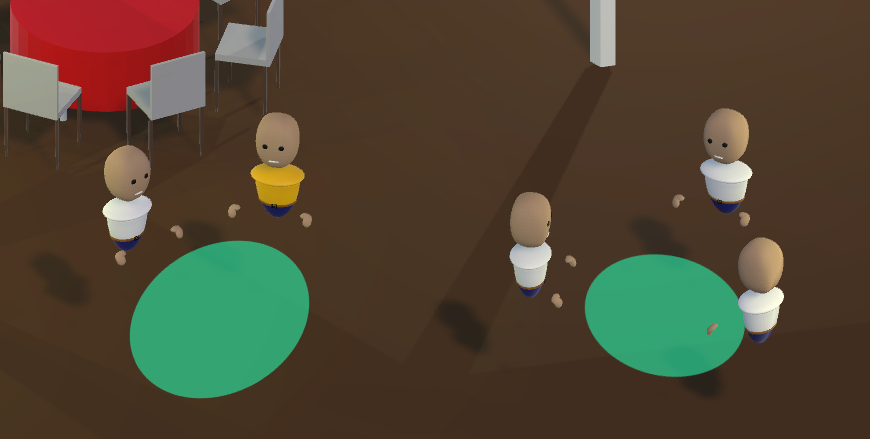
\includegraphics[width=\textwidth]{../graphics/simulator_f_formation.png}
  \caption{F-formation analysis, based on the GCFF algorithm, for 5 Simulator Clients scenario.}
  \label{fig:system:simulator_f_formation}
\end{figure}

The Scene Analysis Server is used to analyze F-formations of the players in the virtual environment, based on their positioning and orientation.
Figure \ref{fig:system:simulator_f_formation} shows an example of F-formation analysis for 5 Simulator Clients scenario.

This server runs a modified version\footnote{Open source and available online at \url{https://github.com/Nagasaki45/gcff}} of the open source Graph-Cuts for F-formation (GCFF) detection algorithm by \cite{Setti2015}.
It is written in \fnurl{Matlab}{https://www.mathworks.com/products/matlab.html} and was recently \fnurl{open sourced}{https://github.com/franzsetti/GCFF}.
Originally developed to analyze still images, the GCFF algorithm detects F-formations using only $(x, y)$ positioning and orientation information in 2 dimensional space.

To integrate it into the system I had to slightly modify the code.
First, as opposed to the original use case, I had to identify F-formations over time.
To illustrate this need, consider a player faking active listening towards an F-formation.
Now, if the other players from that F-formation walk away, the F-formation breaks and the faker shouldn't keep pretending to listen.
It is especially noticeable when other players approaches the place were the faker stands, it should be clear that a new F-formation is formed.
Without the ability to identify F-formations over time the faker won't know that an F-formation broke and that faking active listening is not needed any more.
My implementation of the F-formation tracking over time is based on movement of the F-formations centres.
After each time the GCFF algorithm is called, the new F-formations are compared to the ones that were computed in the previous call.
If the distance of a new F-formation from an old one is bellow an arbitrary threshold, they are considered as the same.
Otherwise, it is a new F-formation.
Second, to be able to call the algorithm from the Main Game Server I wrote a minimal HTTP server in \fnurl{Python}{https://www.python.org/}, that uses \fnurl{Octave}{https://www.gnu.org/software/octave/} and \fnurl{oct2py}{https://github.com/blink1073/oct2py} to invoke the Matlab code.

\section{Active Listening Server}\label{system:active_listening_server}

The Active Listening Server is responsible for predicting backchannel behaviours based on speaker talking state (is speaking or silence) and gaze (is looking at listener or not).
Predicting listeners backchannel behaviours is usually done using either hand-crafted rule based systems, or more recently, data driven and machine learning (ML) approaches \citep{Morency2008}.
Due to the better performance of the later I followed the same path and with the absence of openly available solution decided to develop an ML based backchannel predictor myself.
Using more features, such as prosody \citep{Ward2000} or speaker gestures (TODO reference), could probably improve the model.
However, the simpler model described below was found to be accurate enough.

It is important to note that there is an expected difference in social behaviour between an addressee and a side-participant \citep{Clark1982}.
Although the addressee can fake active listening, in the context of the current research it is more common for side-participants to fake and wonder around, as they are not required to provide verbal response to the speaker.
However, there is much less literature about predicting side-participants active listening behaviours, and even less available resource for training a data-driven model.
With that in mind, I settled for predicting the addressee backchannels and applied them to both addressees and side-participants alike.

Training an ML model required a dataset of conversations with annotations for speaker talking state, gaze, and listener backchannels.
The ICT Rapport Dataset \citep{Gratch2007} contains 126 annotated interactions between a speaker and a listener, and is \fnurl{openly available online}{http://rapport.ict.usc.edu/}, making it ideal for training a backchannel predictor.
Many of the interactions, however, were not properly annotated.
Some of them doesn't contain all of the annotation files while other have blank columns for some of the features of interest.
After filtering out interactions with missing data the remaining 48 interactions had an average length of 138 seconds, ranging from 41 to 248 seconds.

To prepare the data for training I re-sampled the annotations every 100 milliseconds.
Then, to create samples representing a window moving in time I concatenate 30 samples (3 seconds) of the speaker talking state and gaze into one vector.
This vector, when fed into the ML model, should predict the listeners nodding of the last sample.
As a last step of preparation I split the dataset into 3 to 1 train and test portions.

I tried to train three different ML models.
First I attempted to train a Linear Support Vector Machine Classifier (LinearSVC) model using the open source package Scikit-learn \citep{Pedregosa2011}.
Using the test portion of the dataset, the model precision (percentage of correct predictions) was high.
However, the recall (correct predictions out of correct predictions and misses) was very low.
In fact, the model learned to almost never predict a backchannel.
Visually comparing the predictions to the dataset reveals that the it failed to model the data correctly.
Second, I tried to train a Long Short-Term Memory (LSTM) deep neural network with the open source package Keras \citep{Chollet2015}.
The results were similar to these of the LinearSVC model.
Lastly, I trained a K Nearest Neighbors classifier ($K = 5$) with Scikit-learn.
This time, it seems that the model manage to capture nature of the data, as shown in figure \ref{fig:system:backchannel_predictions}.
Using the test portion of the dataset the was lower than before (0.77), but the recall was higher (0.83).

\begin{figure}
  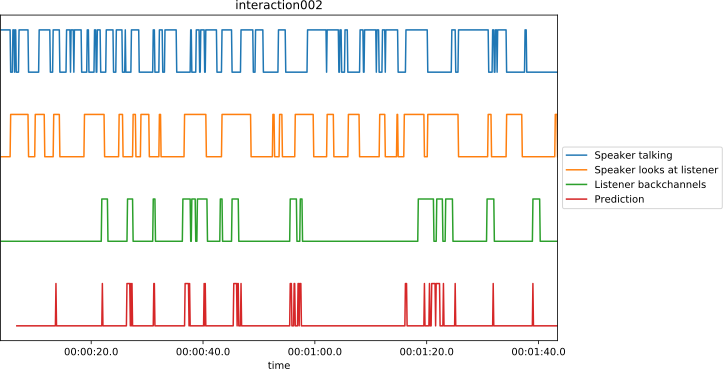
\includegraphics[width=\textwidth]{../graphics/backchannel_predictions.pdf}
  \caption{An example of one interaction between a speaker and a listener from the ICT Rapport dataset, with both actual and predicted listener backchannel behaviours. The lines indicate the state of the features and prediction with values of either 0 when the line is low, or 1 when the line is high.}
  \label{fig:system:backchannel_predictions}
\end{figure}

Choosing between the models didn't follow a properly nor systematic evaluation.
However, based on the performance on the test portion of the dataset and visual inspection the K Nearest Neighbors classifier seemed to performed well enough.
It also provided fast predictions, as necessary by real-time system like this.

To make the backchannel predictions more robust to variations in the input data I implemented the variable threshold as suggested by \cite{Kok2012}.
The K Nearest Neighbors classifier can be used not only to predict a backchannel, as a binary value, but also to predict the probability of a backchannel.
This feature of the model is used, together with a variable threshold to provide predictions.
Initially, the threshold is set to 1, and is decreased over time by 10 percent per second.
When the predicted probability for a backchannel accedes the threshold, a backchannel is predicted and the threshold resets back to 1.

The model, with the variable threshold algorithm, is written in Python and is exposed to the Main Game Server as an HTTP server.
The code for this server is open sourced and \fnurl{available online}{https://github.com/Nagasaki45/backchannel}.

\section{Fake Behaviour Generator}\label{system:fake_behaviour_generator}

The Fake Behaviour Generator integrate the predictions from the Active Listening Sever to provide a smooth and socially appropriate movement for the automated behaviour.
For each participant, the position and orientation of the head and hands, relatively to the chest, is always recorded.
This data is kept in a 2 seconds buffer.
The decision to keep the last 2 seconds is arbitrary and found via trial and error.
This aimed to give a long enough recording to make the faked behaviour look natural, but in the same time not to include two old movements (e.g. when the faker was the speaker or before the F-formation was formed).
When a participant start to fake active listening a playback of this buffer start from the last recorded sample and goes backwards until it reaches the beginning of the buffer, and then forwards again, repeatedly.
This ensure that there are no jumps in the playback of the recorded behaviour.

The chest of an automated active listening agent is always directed to the chest of the speaker in the F-formation.
In case that there is no speaker, the latest speaker is chosen instead.
The chest movement are automated to rotate slowly and smoothly between speakers.

Lastly, the predicted head nods from the Active Listening Server are generating head nods animation that was created in Unity3D.
This animation is merged (position vectors are added together) with the rest of the faked behaviour.


\chapter{Evaluation}\label{evaluation}

The system developed in the current study suggests several interesting evaluation paths.
The first goes back to the comparison with traditional telephony.
Participants in phone conversation can always decide that it's time to end the call.
It is not the same as the decision to stop listening and start doing something else during the phone call.
Therefore, we may assume that when participants fake attention they do so with the intent to keep the conversation going.
This idea is transferable to the virtual environment developed in this study:
Participants can either leave the conversation by walking away, or start faking active listening and do whatever they want.
With that in mind, the system can be used to understand if faking active listening affect the level of conversations, and if so, how.
Extending this idea further, it might be interesting to check how the possibilities exposed by the system affect the overall group dynamics in the cocktail party context.

Another possibility is to add to the extensive research already done in the field of ECAs \citep{Nishimura2007, Bevacqua2008, Gratch2007, Huang2011, Lee2006, Poppe2013}.
Whereas all of these studies assess interaction with an automated agent, in the current study the interaction is with an avatar that switches between human control and automated control.
This difference opens up ways to explore the properties of the transition between the two modes.
More specifically, can the current methods that are used for ECAs can seamlessly replace humans, even for short periods of time?
And more important, what are the limitations of such methods and what can they tell us about active listening behaviours?

Due to the complexity of assessing the level of a conversation, this chapter present the evaluation of the automated active listening properties of the system, with emphasis on the properties of the transition into automated behaviour.
Specifically, I evaluate the time it takes for participants to detect a faked behaviour, the detection accuracy, and the effect of the conversational group size on these measurements.

I Hypothesize that when the size of the conversational group increase it will be harder to notice faked behaviours of side-participants.
I also assume that this will be noticeable to the participants.
Therefore, participants in larger groups will probably use the faked behaviour more frequently.

\section{Pilot}

I ran an unofficial pilot study with 3 co-workers participating during the early development phases of the system.
The faked behaviour at that time was a pre-recorded movement with different time lag between participants to make sure no two fakers look the same.
The pilot attempted to expose user experience issues with the system.
Participants in the pilot were not instructed to do any specific task in the virtual environment, nor fill any questionnaire before or after the experience.
In addition, no measurements were recorded.
Instead, I was interested to hear from the participants about their experience with the system, and probed them to emphasis their experience of the faking mechanism.

The results clearly showed that the transitions into automated behaviour are noticeable.
First, the automated behaviuor didn't responded properly to the social interaction.
This finding are not surprising considering the research in the field of backcahnnel behaviours.
Second, and with equal importance, the change of body posture and the relationship between the body parts between the real and the faked behaviour were significantly noticeable.
Using the hands controllers and the chest tracker, the physical differences between people are recreated in the virtual environment.
In addition, people posture is different, and these differences are also presented in the virtual world.
Ignoring these and using the same behaviour for everyone allowed the participants to learn it quickly and easily notice it.
Much of the design of the Fake Behaviour Generator and the necessity of the Active Listening Server described in \ref{system:fake_behaviour_generator} and \ref{system:active_listening_server} is inspired by these findings.

\section{Methods}

TODO X participants (Y males and Z females) were recruited to the experiment through mailing lists, social media, and prior familiarity (TODO how to describe friends).
The participants were randomly allocated to 3 groups, of 3, 4, and 5 participants.

The participants were asked to participate in a balloon task \citep{Howes2012} in the virtual environment:
They were presented with a scenario of an hot air balloon that is about to crash, unless one passenger will be sacrificed.
They had to come to an agreement, and choose between scarifying a doctor that is about to find a cure for cancer, a 7 months pregnant woman, or her husband, the balloon pilot.
They were also instructed that there are tokens hidden in the virtual environment that they need to find and collect, whilst still progressing towards their shared goal of the balloon task.
To do this they will have to fake participation in the conversation.
Meanwhile, participants in the conversation can accuse others if they think that they are faking active listening by pointing at them and pressing a button on the hand controller.
If a participant is rightfully accused for faking he or she loses one token, but if the accusation is wrong, the accuser loses one token instead.
This mechanism should motivate the participants to maximize the number of tokens they have by the end of the experiment.

Before and after the experience each participant filled a pre and post questionnaires (see appendices \ref{appendix:questionnaire:pre} and \ref{appendix:questionnaire:post} respectively).
The experience itself was conducted in three network connected rooms with audio conference between them using Skype instead of the system voice chat.
Ideally, each participate would be located in a separate room and will use the Vive headset microphone and a pair of headphones.
This ideal solution, however, was not possible due to technical restrictions.
I decided to replace the system voice chat for the experiment with audio conference to prevent participants in the same room to be confused from hearing the others both through the headphones and through the air.

During the experiment the following events were logged and kept for further analysis:

\begin{itemize}
  \item Transitions to and from faked behaviours.
  \item Accusations for faking active listening.
  \item Every time a participant talk with a someone that is faking (the speaker head is directed to the head of a faking participant).
  \item Collection of a token.
\end{itemize}

\section{Results}

\section{Discussion}


\chapter{General discussion}\label{general_discussion}


\chapter{Conclusions}\label{conclusions}

Use VR to investigate new ways of communication, and new social behaviours that are impossible in face to face conversation.

\section{Future work}

Many possible improvements to the idea and implementation.
Faking social behaviour is only one possibility.
Auto swap positioning.

\begin{itemize}
  \item Require attention based on end-of-turn analysis instead of when someone is speaking with me.
  \item Jumping seamlessly between autopilots.
  \item Playback addressee in 4 seconds delay a la \cite{Bailenson2005}.
  \item Train an ML algorithm on VR data, not to predict head nods, but to generate hands and head transforms directly.
\end{itemize}


%%%%%%%%%%%%%%%%%%%%%%%%%%%%%%%%%%%%%%%%%%%%%%%%%%%%%%%%%%%%%%%%%%%%%%%%%%%%%%%%
%% Bibliography:
%%
\cleardoublepage
\phantomsection
\addcontentsline{toc}{chapter}{Bibliography}
\bibliographystyle{plainnat}
\bibliography{thesis}


\begin{appendices}


\chapter{Pre-experience questionnaire}\label{appendix:questionnaire:pre}

\begin{itemize}

\item Participant ID: $\rule{1cm}{0.1mm}$

\item What is your age? $\rule{1cm}{0.1mm}$

\item What is your gender?

\begin{itemize}
  \item Male
  \item Female
  \item Other $\rule{4cm}{0.1mm}$
  \item Prefer not to say
\end{itemize}

\item Have you experienced virtual reality with a head mounted display?

\begin{itemize}
  \item Never
  \item Once
  \item A few times
  \item Regularly
\end{itemize}

\item Have you experienced virtual reality with the HTC Vive?

\begin{itemize}
  \item Never
  \item Once
  \item A few times
  \item Regularly
\end{itemize}

\item Please rate how well you know each of the two other participants.

\begin{tabular}{c|C C C C C}
  & Do not know him/her at all & & & & Know him/her very well \\
  Participant ID $\rule{1cm}{0.1mm}$ & 1 & 2 & 3 & 4 & 5\\
  Participant ID $\rule{1cm}{0.1mm}$ & 1 & 2 & 3 & 4 & 5\\
\end{tabular}

\end{itemize}


\chapter{Post-experience questionnaire}\label{appendix:questionnaire:post}

\begin{itemize}

\item Participant ID: $\rule{1cm}{0.1mm}$

\item What were your strategies to maximize your score?

  \rule{\linewidth}{0.1mm}
  \rule{\linewidth}{0.1mm}
  \rule{\linewidth}{0.1mm}
  \rule{\linewidth}{0.1mm}
  \rule{\linewidth}{0.1mm}
  \rule{\linewidth}{0.1mm}

\item What were your strategies to detect that someone is faking attention?

  \rule{\linewidth}{0.1mm}
  \rule{\linewidth}{0.1mm}
  \rule{\linewidth}{0.1mm}
  \rule{\linewidth}{0.1mm}
  \rule{\linewidth}{0.1mm}
  \rule{\linewidth}{0.1mm}

\item Any other comment?

  \rule{\linewidth}{0.1mm}
  \rule{\linewidth}{0.1mm}
  \rule{\linewidth}{0.1mm}
  \rule{\linewidth}{0.1mm}
  \rule{\linewidth}{0.1mm}
  \rule{\linewidth}{0.1mm}

\end{itemize}


\chapter{Interface}\label{appendix:interface}

\begin{figure}[H]
  \includegraphics[width=\textwidth]{../graphics/interface_manual.pdf}
  \caption{Based on the HTC Vive controllers, the interface allows the players to teleport, fake active listening behaviours, and accuse other players for faking.}
  \label{fig:interface}
\end{figure}


\end{appendices}


\end{document}
